\documentclass[11pt]{article}
\renewcommand{\baselinestretch}{1.20} 
\usepackage[utf8]{inputenc}
\usepackage[english]{babel}
\usepackage{graphicx}
\usepackage{wrapfig}
\usepackage{subcaption}
\usepackage{geometry}
\usepackage{xcolor}
\usepackage{float}
\usepackage{mdframed}
\usepackage{fancyhdr}
\usepackage{lastpage}
\usepackage{booktabs}% http://ctan.org/pkg/booktabs
\newcommand{\tabitem}{~~\llap{\textbullet}~~}
\geometry{a4paper, total={170mm,237mm}, left=20mm, top=20mm}
\setlength{\abovecaptionskip}{15pt plus 3pt minus 2pt}

\pagestyle{fancy}
\fancyhf{}
\rfoot{Side \thepage \hspace{1pt} / \pageref{LastPage}}
\begin{document}
    
    % Title page
    \begin{titlepage}
    \centering
	
\includegraphics[width=0.35\textwidth]{Projectdoc/Assets/Illustrationer/aau_logo_en.pdf}\par\vspace{1cm}
	{\scshape\Large Struktureret System Udvikling\par}
	\vspace{0.2cm}
	{\huge\bfseries Workshop 1\par}
	\vspace{0.2cm}
	{\scshape\Large ITC - B125\par}
	\vspace{2cm}
	{\Large\itshape 
    	Mikkel Steen Hansen\\
        Martin Boe\\
        Benjamin Bach Jensen\\
        Daniel Vestergaard Jensen\\
    \par}
	\vfill
	\vfill
\end{titlepage}
    
    % Table of contents
    \renewcommand{\baselinestretch}{0.8}
    \tableofcontents
    \renewcommand{\baselinestretch}{1.20}
    
    \section{Beskrivelse}
    \textbf{Mini projekt: Vejr station}\\
    Dagens workshop omhandler design af en vejr station til anvendelse i et parcel hus. \\
    Tanken er at forskellige sensorer registrerer en eller flere informationer der skal til for at beskrive
    vejret. Disse data samles op via en enhed der kan videregive information til en app på brugerens smart
    phone, evt. krydret med en præcis vejrudsigt i den kommende time(r) ved at udnytte services fra DMI
    eller anden vejr tjeneste.
    
    \newpage
    
    % First task
    A. Brugeren, Instalatør, alle sensorene og DMI.
En bruger kan altid se indsamlet data, fra enten Sensorene i produktet eller DMI.

En Instalatør vil blive spurgt for en administrator kode inden vedkomende vil få adgang til administrerende settings, så som kalibrering eller data manipulation.

En sensor kan tilgå systemet og tilføje sensor data.

Produktet henter og opdatere data fra DMI hver 15 miniut.

B. Bruger og administrator.


%------------------------------------
\section{Usecase beskrivelse}
\begin{figure}
    \centering
    \includegraphics{}
    \caption{Caption}
    \label{fig:my_label}
\end{figure}
Systemet indeholder som usecase diagrammet anviser fire forskellige aktører:\\
En bruger, der kan få vist den indsamlede data, gennem en af de to mulige grænseflader, for henholdsvis den samlede Sensor data, eller den lokale udsigt opdateret fra DMI.\\
En installatør, der gennem en netbaseret forbindelse kan loggein i systemet, for efterfølgende at administrer produktet, ved f.eks. opsætning eller omkonfigurering, sensor kalibrering, eller datamanipulation.\\
En rakke sensorer der bidrager med forskellige målte data til systemets lokale information, som senere kan fremvises til brugeren.\\
Og en tilgang til DMI's kommende vejrudsigt, der bliver opdateret for brugerens oplevelse.
\\\\
\noindent
Produktets tænkte leveprocess tænkes som:\\
Brugeren køber produktet fra en producent eller distributør.\\
Installerer produktet i sit hjem ved hjælp af den medfølgende manual, og op-kobler produktets hovedmodul til en lokal netværksruter.\\
Efterfølgende kan brugeren tilgå hovedmodulet gennem dens uddelte lokale ipaddresse, fra f.eks. en lokal computer.\\
Igennem denne forbindelse til hovedmodulets, vil brugeren blive guidet gennem en førstegangs opsætnings wizzard.\\
Her efter kan denne forbindelse også bestyres eller konfigurere gennem denne samme tilgang.
    \newpage
    
    % Second Task
    \section{Usecase beskrivelse}

\begin{tabular}{@{}p{3.5cm}@{}p{13cm}@{}}
    Use Case & \#1. Vis data \\
    Description & 
    Bruger(nes) tilgang til systemes, hvor alt samlet data fra systemet tilkoblede sensore kan vises.\\
    Assumtions & 
    Det er antaget at Brugerne og systemet har tilgang til nettet.\\&
    At Usecase \#3 [Samle data] er accepteret,\\&
    og at hovedmodulet har gennemgået en første gangs opsætning.\\
    Actors & 
    Brugere af systemet, med tilgang fra enten app, eller net forbindelse \\
    Steps & For visning af data skal brugeren:
    \begin{enumerate}
        \item forbinde til systemet med app.
        \item Vælge at se målte sensor data fra hovedmenu.
    \end{enumerate} \\&
    Systemet gennemgår herefter:
    \begin{enumerate}
        \item At hente lokalt gemt data fra sensor(ene)
        \item Fremvise dataen i app for brugeren.
    \end{enumerate}\\
    Variations & 
    Forskellige layouts alt efter antal af tilkoblede sensorer.\\&
    Responsivedesign for mobil, tablet og computer.\\
    Non-Funtional & 
    \tabitem Brugeren kan kun se de nyeste beregnede informationer.\\&
    \tabitem Brugeren skal ikke kunne redigere eller på anden måde manipulere, lokalt data.
\end{tabular}
\\\\

\noindent
\begin{tabular}{@{}p{3.5cm}@{}p{13cm}@{}}
    Use Case & \#2. Login \\
    Description &  
    Denne use case skal bruges for at kunne identificere sig over for systemet som installatør. Formålet med dette er at afskærme brugeren fra funktioner som ikke skal bruges i hverdagen.\\
    Assumtions &  
    Det er antaget at systemet er tilkoblet både strøm og internet\\
    Actors & 
    Installatør af systemet, med tilgang fra en lokal computer.\\
    Steps & 
    \begin{enumerate}
        \item Installatør bedes om login detaljer
        \item Systemet verificerer login detaljer
        \item Ved godtagelse sendes installatør til konfigurationsmenu.
    \end{enumerate}\\
    Variations & 
    Systemet har ikke gennem gået en første gangs opsætning, og kræver derfor opsætnings wizzard.
    Forbindelsen findes spæret, forsøg på uautoriseret adgang.\\
    Non-Functional &
    Login efter første gangs opsætning, skal ikke findes nødvendigt.\\ &
    Efter 5 mislykkedes login forsøg, vil forbindelsen blive spæret.
\end{tabular}
\\\\

\noindent
\begin{tabular}{@{}p{3.5cm}@{}p{13cm}@{}}
    Use Case & \#3. Samle data \\
    Description & 
    Denne use case skal indsamle data fra de tilgængelige sensorer samt DMIs database. Formålet med dette er, at gøre denne data tilgængelig for andre use cases, så som Use case \#1. (Vis data).\\
    Assumptions & 
    Det er antaget at use casen "Konfigurering" er gennemført samt at "Kalibrering af sensorer" use casen er gennemført for alle tilkoblet sensorer. Det antages dernæst også at systemet har tilgang til internettet.\\
    Actors & 
    Denne use case involverer to aktører, de tilkoblet sensorer og DMIs database.\\
    Steps & 
    Gentages hvert femte minut:
    \begin{enumerate}
        \item Sensorer kontaktes for data udlæsning
        \item Udlæst data gemmes i lokal database
    \end{enumerate}\\ &
    Gentages hvert kvarter:
    \begin{enumerate}
        \item DMIs database kontaktes for lokal vejr opdatering
        \item Ny data sammenlignes med gammel data i lokal database.
        \item Ny data overskriver gammel data, hvis de to ikke er ens.
    \end{enumerate}\\ 
    Variations & 
    DMI er ikke tilgængelig.\\
    Non-Functional & 
    Systemet skal kunne fortsat operere i lokal tilstand hvis DMIs database ikke kan kontaktes\\
\end{tabular}
    \newpage
    
    % Third Task
    \section{Kravspecifikation}
På baggrund af de før specificerende Usecase, defineres følgende krav til produktet:
\begin{itemize}
    \item Produktet skal kunne tilsluttes ethernet.
    \item Produktet skal kunne tilgås gennem en konfigurations net-port.
    \item Produktet skal kunne finde og skabe forbindelser til enkelte sensorer(moduler).
    \\
    \item Brugeren skal kunne tilgå produktets data gennem et interface.
    \item Brugeren skal kunne se data fra alle tilkoblede sensorer.
    \item Brugere skal ikke kunne manipulere fremvist data.
    \item Brugere skal kunne tilgå sensor data så længe der forefindes internet forbindelse.
    \\
    \item En installatør skal kunne konfigurér produktet så længe der forefindes internet forbindelse.
    \item En installatør skal kunne manipulere lokalt indsamlet data i form af sletning (Clearing).
    \item En installatør skal altid manuelt / fysisk kunne gendanne til fabriks indstillinger.
    \\
    \item En sensor skal separat kunne oprette forbindelse til et hovedmodul.
    \item Hovedmodulet skal kunne forbinde og indsamle nyeste data fra DMI.
    \item En sensor skal kunne oplagre information lokalt på hovedmodulet.
\end{itemize}


    \newpage
    
    % Fourth Task.
    \begin{figure}[H]
    \centering
    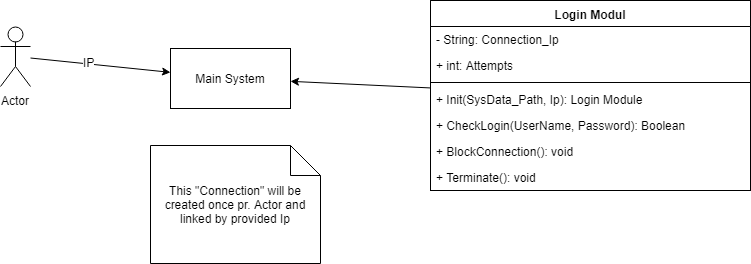
\includegraphics[width=1\linewidth, height=6cm]{Struktureret_System_Udvikling/Workshop_1/Assets/ClassDiagram.png}
    \caption{Class Diagram}
    \label{fig:my_label}
\end{figure}

\noindent
\\Som ses på ovenstående diagram har gruppen valgt en af de førnævnte use cases, til en nærmere beskrivelse. i dette tilfælde er der valgt use case \#2. Login.
Denne indeholder 2 moduler, navngivet CheckLogin og BlockConnection, foruden de 2 fastsatte, henholdvis constructor og destroyer. Idéen bag denne implementation er at modulet initieres for hver forsøgende forbindelse, identificeret via den forbindende kontakts ip-addresse. Foruden denne ip initieres modulet også med en given path, til en system fil indeholdende systemets login kriterier, og en liste over blokerede ip'er.
Her efter kan CheckLogin anvendes til at checke om et set loginoplysninger fra den forbindende bruger er sand, da denne returnere sand ved korrekte loginoplysninger. Samtidigt kan denne også bruges til at fange mulige angreb da hvis de angivne oplysninger ikke er sande, vil modulets interne tæller "Attempts" tælle op, og derfor vil denne kunne anvendes til at identificere eventuelle angreb.
Ved identifikation af et sådant angreb vil BlockConnection herefter kunne tilføje modulets initierede forbindelses ip til listen i systemfilerne over blokerede forbindelser.
Og tilsidst kan modulet Terminieres.

\noindent
\\For Usecase #2. Login\\
Ville Overstående Modul skulle anvendes i følgende sammenhæng:\\
\noindent
0. Check if connecting IP is part off blocklist, from SysData
\\1. Init()\\
- With path to lib providing sys kalibrated data\\
- And the connection IP\\
- Init returns error if provided connection Ip is part of Block List
\\2. CheckLogin()\\
- With User provided login credentials\\
3.1 If CheckLogin returns False:\\
- If Attempts for current connection Module more than 5 BlockConnection()\\
3.2 If CheckLogin returns True:\\
- Send user to administration page (Login is done) \\
4. Terminate()
    
    % Fifth Task.
    %\input{}
\end{document}